\chapter{Simplicial Sets}

\section{Introduction}

A {\em simplicial set}{\footnote {{\bf Hilton \&  Wylie}, {\em Homology theory}, Cambridge University Press, 1967}}
$K$ is a union $K={\displaystyle{\bigcup_{q\ge 0}{K^q}}}$, where the $K^q$ 
are disjoints sets, together with functions\index{simplicial sets}
$$\partial_i^q: K^q \longrightarrow K^{q-1},\quad q>0,\quad i=0,\ldots , q,$$
$$\eta_i^q: K^q \longrightarrow K^{q+1},\quad q\ge 0,\quad i=0,\ldots ,q,$$
subject to the relations
$$\diagram{
\partial_i^{q-1}\partial_j^q   & = & \partial_{j-1}^{q-1}\partial_i^q, &   i < j \cr
\eta_i^{q+1}\eta_j^q       & = & \eta_j^{q+1}\eta_{i-1}^q,    & i > j    \cr
\partial_i^{q+1}\eta_j^q     & = & \eta_{j-1}^{q-1}\partial_i^q,   & i < j  \cr
\partial_i^{q+1}\eta_i^q     & = & \partial_{i+1}^{q+1}\eta_i^q    & Identity,   \cr
\partial_i^{q+1}\eta_j^q     & = & \eta_j^{q-1}\partial_{i-1}^q,   &  i > j+1.\cr 
}$$
An element of $K^q$ is an ({\em abstract}) $q$--simplex of $K$ and the functions $\partial$ and $\eta$ are
respectively the {\em face operators}\index{operator!face} 
and the {\em degeneracy operators}\index{operator!degeneracy}. Formally, their action 
on a simplex is very simple. For instance, if a $q$--simplex is an ordered set of vertices, like
$\lbrace v_0, v_1, \ldots,v_i,\ldots, v_q \rbrace$, 
the rules are the following (we omit the indication of the dimension of the simplex):
\begin{eqnarray*}
\partial_i \lbrace v_0, v_1, \ldots,v_i,\ldots, v_q \rbrace & = &
           \lbrace v_0, v_1, \ldots,{\bf v_{i-1}}, {\bf v_{i+1}},\ldots, v_q \rbrace, \\
\eta_i \lbrace v_0, v_1, \ldots,v_i,\ldots, v_q \rbrace & = &
      \lbrace v_0, v_1, \ldots,{\bf v_i},{\bf v_i},\ldots, v_q \rbrace.
\end{eqnarray*}
The operators $\partial_i^q$ will be used hereafter to define the boundary operator $d^q$
for the $q$--component of the associated chain complex:
$$d^q = \sum_{i=0}^q { (-1)^i \partial_i^q}.$$
The image of a simplex under some $\eta$ is called {\em degenerate}, because it
is not directly implied  in the realization of the simplicial set.

\subsection* {Example}

Let us take the small example {\em diabolo} from the chapter 1.
For a better understanding, it is convenient to use a list representation for the
simplices. So the set $K^0$ of $0$--simplices (vertices) is:
$$\lbrace (0), (1),\ldots (5) \rbrace.$$
The set $K^1$ of $1$--simplices contains the set of regular simplices:
$$\lbrace (0\  1), (0\  2), (1\  2), (2\  3), (3\  4), (3\  5), (4\  5) \rbrace,$$
but also the degenerate $1$-- simplices:
$$\lbrace (0\ 0), (1\ 1), (2\ 2),\ldots,(5 \ 5) \rbrace.$$
The set $K^2$ of $2$--simplices contains the regular singleton:  
$$\lbrace ( 3\  4\  5) \rbrace$$
but also the degenerate $2$--simplices:
$$\lbrace (0\ 0\ 0), \ldots, (5\ 5\ 5), (0\ 0\ 1), (0\ 0\  2), (1\ 1\ 2), \ldots, (4\ 5\ 5)\rbrace.$$
The sets $K^q$ ($q >2$) contain only degenerate simplices.
With this  naming of the elements of a $q$--simplex, the action of $\partial$ and $\eta$ is now clear. For
instance
$$\partial_0 (0\  1) = (1),\  \partial_1 (0\  1) = (0),$$
$$\eta_0 (0\  1) = (0\  0\  1),\ 
  \eta_1 (1\  2)= (1\  2\  2),\ \eta_2(3\ 4\ 5)=(3\ 4\ 5\ 5). $$
By the way, we see that a simplex is non-degenerate if the list is strictly increasing.

\section {Notion of abstract simplex in this Lisp implementation}

In\index{simplex!abstract} this implementation, 
on account of the essential following property: {\em any simplex
may be expressed in an unique way as a possibly iterated degeneracy of a non--degenerate
simplex}, we call an {\bf abstract simplex}, (in short {\bf absm}), a pair consisting of:
\begin{itemize}
\item a (possibly iterated) degeneracy operator,
\item a ``geometric'' simplex, i.e. a non--degenerate simplex\index{simplex!geometric}.
\end{itemize}
For instance, if $\sigma$ is a non--degenerate simplex, and $\sigma'$ is the degenerate simplex 
$\eta_3\eta_1\sigma$, the corresponding abstract simplices are respectively 
$\lbrace \emptyset, \sigma \rbrace$ and $\lbrace \eta_3\eta_1, \sigma \rbrace$.
\par
An abstract simplex is represented internally in the system by the following lisp object:
\begin{center}
{\tt (:absm {\em dgop} . {\em gmsm})}
\end{center}
where,
\begin{enumerate}
\item {\em dgop} is a non-negative integer coding\index{simplex!coding} 
a {\em strictly decreasing integer list}. 
This strictly  decreasing list of integers represents a sequence
of $\eta$ o\-pe\-ra\-tors and is coded as a {\bf unique} integer with the following convention: a number $i$ in
the sequence is the $i+1$--th binary bit of a machine word. The null list is coded as the number $0$ whereas
the list {\tt (0)}, i.e. the $\eta_0$ operator, is coded as the integer {\tt 1}, etc.
Two functions are provided to help the user for the transformation in both directions.
\item {\em gmsm} is a geometric simplex,  i.e. any kind lisp object   modelizing a non--degenerate 
simplex. For practical reason, a  type {\tt GMSM}, (any kind of lisp object), has been defined.
\end{enumerate}
The simplest constructor is the macro  {\tt (absm (dgop-ext-int {\em dgop-list}) {\em gmsm})}, 
where {\em dgop-list} is a strictly decreasing integer list. A type {\tt ABSM} has been defined.
The associated printing method prints such an object under the form:
\begin{center}
{\tt <AbSm {\em ext-dgop gmsm}>}
\end{center}
where {\em ext-dgop} shows clearly the sequence of the operators $\eta_i$ (see the e\-xam\-ples).
The accessor functions for the components are the macros {\tt dgop} and {\tt gmsm}.
\newpage

\subsection {Simple functions for abstract simplices}

{\parindent=0mm
{\leftskip=5mm 
{\tt dgop-ext-int} {\em ext-dgop} \hfill {\em [Function]}\par}
{\leftskip=15mm 
Code on an integer the valid list representing the degeneracy o\-pe\-ra\-tor {\em ext-dgop}. \par}
{\leftskip=5mm 
{\tt dgop-int-ext} {\em dgop} \hfill {\em [Function]}\par}
{\leftskip=15mm 
Give the list representing a degeneracy operator from the integer {\em dgop}. \par}
{\leftskip=5mm 
{\tt absm} {\em dgop gmsm} \hfill {\em [Macro]}\par}
{\leftskip=15mm 
Create an abstract simplex, using directly the coded representation, {\em dgop}, of the degeneracy operator. \par}
{\leftskip=5mm 
{\tt dgop} {\em absm} \hfill {\em [Macro]}\par}
{\leftskip=15mm 
Get the integer code of the internal representation of the degeneracy operator of the
abstract simplex {\em absm}. \par}
{\leftskip=5mm 
{\tt gmsm} {\em absm} \hfill {\em [Macro]}\par}
{\leftskip=15mm 
Get the basic non-degenerate simplex part of the abstract simplex {\tt absm}. \par}
{\leftskip=5mm 
{\tt absm-p} {\em object} \hfill {\em [Predicate]}\par}
{\leftskip=15mm 
Test if {\em object} is an abstract simplex. \par}
}

\subsection* {Examples} 

Let us suppose that {\tt :sigma} ``is'' a geometric simplex,
we may construct the abstract simplices of the beginning of the section.
{\footnotesize\begin{verbatim}
(dgop-ext-int '(0) )  ==>

1

(dgop-ext-int '(4 0) )  ==>

17

(dgop-int-ext 63)  ==>

(5 4 3 2 1 0)

(dgop-ext-int '(2 2))  ==>

Error: In DGOP-EXT-INT, the external dgop (2 2) is not decreasing.

(setf asigma (absm 0 :sigma)) ==>

<AbSm - SIGMA>

(setf asigma-prime (absm (dgop-ext-int '(3 1)) :sigma)) ==>

<AbSm 3-1 SIGMA>

(absm-p asigma-prime)  ==>

T
\end{verbatim}}
The following  command gives
the sixth degeneracy of the vertex $0$ represented as {\tt (0)}.
{\footnotesize\begin{verbatim}
(setf deg-6 (absm (dgop-ext-int '(5 4 3 2 1 0)) '(0)))  ==>

<AbSm 5-4-3-2-1-0 (0)>

(dgop deg-6)  ==>

63

(gmsm deg-6)  ==>

(0)

\end{verbatim}}


\section {Representation of a simplicial set}

A simplicial set\index{class!{\tt SIMPLICIAL-SET}} is implemented as an instance of the 
class  {\tt SIMPLICIAL-SET}, subclass of the class {\tt COALGEBRA}.
{\footnotesize\begin{verbatim}
(DEFCLASS SIMPLICIAL-SET (coalgebra)
    ((face :type face :initarg :face :reader face1)))
\end{verbatim}}
This class inherits also from the class {\tt CHAIN-COMPLEX} and has one slot of its own:
\begin{description}
\item {{\tt face}}, a lisp function  computing any face of any geometric simplex of the simplicial set.
This is a function with $3$ arguments: a face index (a non--negative integer, {\tt indx}), a simplex dimension
(a positive integer, {\tt dmns}) and a geometric simplex ({\tt gmsm}), the $indx$--th face of which
is looked for. Whatever the face simplex is, degenerate or not, the simplex returned by this function
must be an {\bf abstract} simplex, i.e. an {\tt ABSM} object.
\end{description}
A printing method has been associated to the class {\tt SIMPLICIAL-SET} 
and the external representation of  an instance is a string like {\tt [K{\em n} Simplicial-Set]}, where $n$
is the number plate of the Kenzo object. 

\section {The function build-smst}

To\index{function!{\tt build-smst}} facilitate the construction of instances of the 
class {\tt SIMPLICIAL-SET}, the software {\tt Kenzo} provides the function {\tt build-smst}
defined with keyword parameters:
\vskip 0.40cm
{\tt build-smst}\par
\hspace {1cm}{\tt :cmpr} {\em cmpr} {\tt basis} {\em basis} {\tt :bspn} {\em bspn} {\tt :face} {\em face} \par
\hspace {1cm}{\tt :face*} {\em face*} {\tt :intr-bndr} {\em intr-bndr} {\tt :bndr-strt} {\em bndr-strt} \par
\hspace {1cm}{\tt :intr-dgnl} {\em intr-dgnl}  {\tt :dgnl-strt} {\em dgnl-strt }{\tt :orgn} {\em orgn}
\vskip 0.40cm
The returned value is an object of type {\tt SIMPLICIAL-SET}. 
This function assigns an identification number {\tt idnm} to the Kenzo object instance in
a sequential way and pushes this object on the list of already  created simplicial sets instances, {\tt *smst-list*}.
\par
The keywords parameters are:
\begin{itemize}
\item [--] {\em cmpr}, a comparison function for generators. 
\item[--] {\em basis}, if the simplicial set is effective, this argument must be the lisp function 
returning the  list of non-degenerate simplices  of the simplicial set, in a given dimension; 
if the simplicial set is locally effective, this argument must be the keyword {\tt :locally-effective}.
\item[--] {\em bspn}, the lisp representation of the base point (an item of type {\tt GMSM}). This is
in fact the slot {\tt bsgn} of the associated chain complex.
\item[--] {\em face}, a lisp function for the face operators.
\item[--] {\em face*}, a lisp function for the face operators, returning the symbol {\tt :degenerate} if
the corresponding face is degenerate.
\item[--] {\em intr-bndr}, a lisp function for the differential of the associated chain complex.
\item[--] {\em bndr-strt}, the strategy ({\tt :cmbn} or {\tt :gnrt}) for the function {\em intr-bndr}.
\item[--] {\em intr-dgnl}, a lisp function for the coproduct of the coalgebra.
\item[--] {\em dngl-strt}, the strategy ({\tt :cmbn} or {\tt :gnrt}) for the function {\em intr-dgnl}.
\item[--] {\em org}, the comment list, adequately chosen.
\end{itemize}

The three arguments {\em face*},  {\em intr-bndr} and {\em intr-dgnl} are not mandatory.
Only the function {\em face} is necessary to define precisely the simplicial set.
From the function {\em face}, we know that we may construct:
\begin{itemize} 
\item The differential for the associated chain complex,
according to the formula :
$$d^q = \sum_{i=0}^q { (-1)^i \partial_i^q}.$$
\item The coproduct of the underlying coalgebra (the Alexander-Whitney diagonal, $\Delta$) according to the
formula:
$$\Delta(\sigma)= \sum_{i=0}^{n}{{\tilde{\delta}}^{(i)}\sigma \otimes \delta_0^{(i)} \sigma},$$
where the power $(i)$ denotes the $i$-th composition of the operator and $\tilde{\delta}$ is the
{\em last face} operator, so that $${\tilde{\delta}}^{(i)}=\delta_{n-i+1}\circ \cdots \circ \delta_{n-1}\circ \delta_n.$$
\end{itemize}
But, as the differential ignore degenerate faces, it may be interesting for the user to provide a face function,
weaker than the function {\em face} but sufficient and more efficient to compute the boundary of a
simplex. It is the raison d'\^etre of the parameter {\em face*} which may be used as an alternative to {\em face}.
In both cases, the strategy is set to {\tt :gnrt} by the system. It may also arrive that the user knows
a particularly simple form for the differential, he may then use the parameter {\em intr-bndr}. In the computation
of differentials in the associated chain complex, this function will be used instead of the
canonical differential computed from the face function. In this last case, the user is required to provide
the strategy. Same remark for the parameter {\em intr-dgnl}.

\subsection* {Examples}

As first example, we give the construction of the simplicial set $\Delta^n$  cor\-res\-pon\-ding to the 
standard $n$-simplex. This is given only as example. The program {\tt Kenzo} provides a function
for the same purpose which will be described later.
For every simplex, we shall use a list representation as in our first example {\tt diabolo}. The various 
keyword arguments for the call to {\tt build-smst}, are:
\newpage
\begin{enumerate}
\item {\em bspn}, the list {\tt (0)}, i.e. the representation of the vertex $0$.
\item {\em cmpr}, the lisp function  {\tt \#'l-cmpr}, since this function is adequate to compare the
lists representing the simplices.
\item {\em basis}, the lisp function returning the list of all possible 
non--degenerate simplices in some dimension. Here, this is the combinatory function returning the set 
of all the lists of $p+1$ objects taken among $n+1$. 
Such a function is for instance the function  ({\tt delta-inj} {\em p n}) whose definition is given
hereafter. So, the  {\tt :basis} keyword argument is simply:
\par {\footnotesize\tt \#'(lambda(dmn) (delta-inj dmn n))}.
\par
Note that here, {\tt n} is a global parameter.
\item  {\em face}, the lisp function for the face operators ({\tt face-delta-n}). It consists simply in
removing the $i$--th element of the list describing a simplex ($i$ starting at $0$).
\item  {\em org} will be a comment.
\end{enumerate}

{\footnotesize \begin{verbatim}
(defun delta-inj (m n)
  (declare (type fixnum m n))
  (cond ((> m n) +empty-list+)
        ((zerop m) (mapcar #'list (<a-b> 0 n)))
        (t (mapcan #'(lambda (list)
                       (declare (type list list))
                       (mapcar #'(lambda (k)
                                   (declare (type fixnum k))
                                   (cons k list))
                                 (<a-b< 0 (first list))))
                     (delta-inj (1- m) n)))))

(delta-inj 0 3) ==>

((0) (1) (2) (3))

(delta-inj 1 3)  ==>

((0 1) (0 2) (0 3) (1 2) (1 3) (2 3))

(delta-inj 3 3)  ==>

((0 1 2 3))

(setf face-delta-n
  #'(lambda(i dmn gsm)
      (declare(ignore dmn))
      (absm 0 (append (subseq gsm 0 i)
                      (subseq gsm (1+ i))) )))
\end{verbatim}}
To create $\Delta^n$ for any order $n$, we embed the call of {\tt build-smst} in a function having
$n$ as parameter. 
{\footnotesize \begin{verbatim}
(defun delta-n(n)
  (declare (type fixnum n))
        (build-smst :cmpr #'l-cmpr
                    :basis #'(lambda(dmn)(delta-inj dmn n))
                    :bspn '(0)
                    :face face-delta-n
                    :orgn `(delta-n ,n)))    ==>

DELTA-N

(setf delta4 (delta-n 4))  ==>

[K3 Simplicial-Set]

(bspn delta4)  ==>

(0)

(basis delta4 0)  ==>

((0) (1) (2) (3) (4))

(basis delta4 3)  ==>

((0 1 2 3) (0 1 2 4) (0 1 3 4) (0 2 3 4) (1 2 3 4))
\end{verbatim}}
\vskip 0.40cm
A second example is the contruction of the simplicial complex  $\Delta^{\N}$ freely generated 
by the positive integers. The construction of the {\tt SIMPLICIAL-SET} instance to implement this
simplicial set is quite similar to that of $\Delta^n$, but in this case the {\tt :basis} keyword
argument is  the keyword {\tt :locally-effective}, since the sets $K^q$ are infinite. Whence,
the definition of $\Delta^{\N}$:
{\footnotesize\begin{verbatim}
(setf delta-infty
        (build-smst :cmpr #'l-cmpr
                    :basis :locally-effective
                    :bspn '(0)
                    :face face-delta-n
                    :orgn `(delta-infinity)))
\end{verbatim}}
\vskip 0.40cm
A third example is the construction of the simplicial set corresponding to  {\tt diabolo}. This 
simplicial set is a  sub--complex of $\Delta^2$.
The {\tt :face} function is exactly the same as in the examples above and the {\tt :basis} function returns
the sub--simplices of {\tt diabolo}, by enumeration. 
{\footnotesize \begin{verbatim}
(setf diabolo-ss 
        (build-smst :cmpr #'l-cmpr
                    :basis  #'(lambda (dmn)
                                (case dmn
                                      (0 '((0)(1)(2)(3)(4)(5)))
                                      (1 '((0 1)(0 2)(1 2)(2 3)(3 4)(3 5)(4 5)))
                                      (2 '((3 4 5)))))
                    :bspn '(0)
                    :face face-delta-n
                    :orgn '(simplicial set for diabolo)))
\end{verbatim}}
\newpage

\section {A first set of helpful functions on simplicial sets}

We give now a first set of functions, methods or macros acting on  simplicial set instances. 
\vskip 0.45cm
{\parindent=0mm
{\leftskip=5mm
{\tt cat-init} \hfill {\em [Function]} \par}
{\leftskip=15mm
Clear in particular {\tt *smst-list*}, the list of user created simplicial sets  and reset
the global counter to $1$. \par}
{\leftskip=5mm 
{\tt smst} {\em n} \hfill {\em [Function]}\par}
{\leftskip=15mm 
Retrieve in the list {\tt *smst-list*} the simplicial set instance whose the Kenzo identification
is $n$. If it does not exist, return {\tt NIL}. \par}
{\leftskip=5mm 
{\tt cmpr} {\em smst  absm1 absm2} \hfill {\em [Macro]}\par}
{\leftskip=15mm 
Compare the abstract simplices {\em absm1} and {\em absm2} with the comparison function
associated with the simplicial set {\em smst}. \par}
{\leftskip=5mm 
{\tt bspn} {\em smst} \hfill {\em [Macro]}\par}
{\leftskip=15mm 
Return the base point of the simplicial set {\em smst}. \par}
{\leftskip=5mm 
{\tt bndr}  {\em smst} {\tt \&rest} \hfill {\em [Macro]}\par}
{\leftskip=15mm 
Identical to the macro {\tt dffr} (see the chain complex chapter). For simplicial sets, it is more traditional to
use the term {\em boundary}. \par}
{\leftskip=5mm 
{\tt dgnl} {\em smst} {\tt \&rest} \hfill {\em [Macro]}\par}
{\leftskip=15mm 
Identical to  the macro {\tt cprd} (see the coalgebra chapter). For simplicial sets, this recalls the 
Alexander-Witney diagonal. \par}
{\leftskip=5mm 
{\tt face} {\em smst i k  gmsm-or-absm} \hfill {\em [Macro]}\par}
{\leftskip=15mm 
Versatile macro to apply the face operator $\partial_i^k$ on the   simplex {\em gmsm-or-absm} of the simplicial set
{\em smst}. The name of the simplex parameter
shows clearly that it may be either a geometric simplex or an abstract simplex. 
With only one argument ({\em smst}), return the function {\em face}. 
In any other case, we recall that this application   returns always  an object of type {\tt ABSM}. \par}
{\leftskip=5mm 
{\tt degenerate-p} {\em  absm} \hfill {\em [Macro]} \par}
{\leftskip=15mm 
Return {\tt t} if the abstract simplex {\em asm} is degenerate, {\tt nil} otherwise. \par}
{\leftskip=5mm 
{\tt non-degenerate-p} {\em  absm} \hfill {\em [Macro]} \par}
{\leftskip=15mm 
Return {\tt t} if the abstract simplex {\em asm} is non-degenerate, {\tt nil} otherwise. \par}
{\leftskip=5mm 
{\tt check-smst} {\em smst dmns1 {\tt \&optional} dmns2 (1+ dmns1)} \hfill {\em [Function]}  \par}
{\leftskip=15mm 
Return {\tt t} if the fundamental relations between the face operators $\partial_i^k$
with $k=dmns1,\ldots, dmns2-1$,
applied on the effective simplicial set {\em smst}, are satisfied, otherwise {\tt nil}.
If the optional parameter {\em dmns2} is omitted, the test is done only for
$k=dmns1$. \par}
}

\subsection* {Examples}
After having created instances of the standard simplicial sets $\Delta^2$ and $\Delta^3$ 
($\Delta^{\N}$ has been defined previously), let us test some simple functions. 
Note that, since the class of simplicial sets is a sub-class of the class of coalgebras, 
itself subclass of chain complexes, 
the functions defined on these classes are available.
{\footnotesize\begin{verbatim}
(setf delta2 (delta-n 2))  ==>

[K8 Simplicial-Set]

(setf delta3 (delta-n 3))  ==>

[K9 Simplicial-Set]

(degenerate-p (absm 0 '(1 2 3)))  ==>

NIL

(degenerate-p (absm 5 '(0 1 2 3 4)))  ==>

T

(basis delta3 2)  ==>

((0 1 2) (0 1 3) (0 2 3) (1 2 3))

(basis delta2 0)  ==>

((0) (1) (2))
\end{verbatim}}
The set of simplices in any dimension for the simplicial set $\Delta^\N$ is infinite:
{\footnotesize\begin{verbatim}
(basis delta-infty 1)  ==>

Error: The object [K3 Simplicial-Set] is locally-effective.
\end{verbatim}}
Let us test the face function. We see that, though {\tt delta-infty} is locally effective,
nevertheless, we may work with its simplices:
{\footnotesize\begin{verbatim}
(face delta-infty 2 4 '(0 1 2 3 4))  ==>

<AbSm - (0 1 3 4)>

(face delta-infty 2 4 (absm 0 '(0 1 2 3 4)))  ==>

<AbSm - (0 1 3 4)>

(face delta-infty 2 5 (absm (dgop-ext-int '(1)) '(0 1 2 3 4)))  ==>

<AbSm - (0 1 2 3 4)>

(face delta-infty 2 5 (absm (dgop-ext-int '(3)) '(0 1 2 3 4)))  ==>

<AbSm 2 (0 1 3 4)>

(bspn delta-infty)  ==>

(0)
\end{verbatim}}
The two following statement show that {\tt delta-infty} may be considered
also as a coalgebra and a chain complex.
{\footnotesize\begin{verbatim}
(cprd delta-infty 4 '(0 1 2 3 4))  ==>

----------------------------------------------------------------------{CMBN 4}
<1 * <TnPr (0) (0 1 2 3 4)>>
<1 * <TnPr (0 1) (1 2 3 4)>>
<1 * <TnPr (0 1 2) (2 3 4)>>
<1 * <TnPr (0 1 2 3) (3 4)>>
<1 * <TnPr (0 1 2 3 4) (4)>>
------------------------------------------------------------------------------

(? delta-infty 4 '(0 1 2 3 4))  ==>

----------------------------------------------------------------------{CMBN 3}
<1 * (0 1 2 3)>
<-1 * (0 1 2 4)>
<1 * (0 1 3 4)>
<-1 * (0 2 3 4)>
<1 * (1 2 3 4)>
------------------------------------------------------------------------------

\end{verbatim}}
The simplicial set {\tt diabolo-ss},  has also all the properties of a coalgebra and
of a chain complex.
{\footnotesize\begin{verbatim}
(basis diabolo-ss 1)  ==>

((0 1) (0 2) (1 2) (2 3) (3 4) (3 5) (4 5))

(basis diabolo-ss 2)  ==>

((3 4 5))

(? diabolo-ss 2 (first *))  ==>

-----------------------------------------------------------------------{CMB 1}
<1 * (3 4)>
<-1 * (3 5)>
<1 * (4 5)>
------------------------------------------------------------------------------

(? diabolo-ss *)  ==>

----------------------------------------------------------------------{CMBN 0}
------------------------------------------------------------------------------

(dgnl diabolo-ss **)  ==>

----------------------------------------------------------------------{CMBN 1}
<1 * <TnPr (3) (3 4)>>
<-1 * <TnPr (3) (3 5)>>
<1 * <TnPr (4) (4 5)>>
<1 * <TnPr (3 4) (4)>>
<-1 * <TnPr (3 5) (5)>>
<1 * <TnPr (4 5) (5)>>
------------------------------------------------------------------------------

\end{verbatim}}

\newpage

\section{The function build-finite-ss}

The\index{function!{\tt build-finite-ss}} function {\tt build-finite-ss} 
is a powerful function simplifying the creation of a finite
simplicial set. From the lisp point of view, it accepts only one argument, the structured list
of the simplices and their faces. In this list, every non--degenerate simplex must
be coded as a symbol given by the user.  The  structure of the list is the following:
\begin{itemize}
\item {\bf 0}    (in fact, optional)
\item $<$Sequence of the vertices, the first item being the base point$>$,
\item {\bf 1}
\item $<$Sequence of description of simplices in dimension 1$>$,
\item {\bf 2}
\item $<$Sequence of description of simplices in dimension 2$>$,
\item   ... ... ... ... ... ...
\item {\bf n}
\item $<$Sequence of description of simplices in dimension n$>$.
\end{itemize}
where $<$Sequence of description of simplices in dimension k$>$ is a sequence of
the following items:
\begin{enumerate}
\item A symbol, the symbolic name of the simplex.
\item A list of  faces of this simplex, describing the faces of the simplex.
A face can be described in two ways:
\begin{itemize}
\item [--] a symbol, the symbolic name of a {\bf non-degenerate} simplex composing itself the
face.
\item [--] or a list of the form  ($i_k\ i_{k-1}\ \ldots \ i_1 \ i_0$ {\tt symbol}) meaning that the degeneracy
$\eta_{i_k}\eta_{i_{k-1}}\ldots\eta_{i_1}\eta_{i_0}$ is to be applied to the non-degenerate simplex
of name {\tt symbol}  to produce the actual (possibly degenerate) face. If the simplex face has dimension $0$ (a vertex), 
the name of this vertex is sufficient in the
face description because the program computes itself
the unique possible degeneracy of the vertex, i.e. $\eta_{k-2}\ldots\eta_0$. 
\end{itemize}

\end{enumerate}
\subsection* {Examples}
Let us give some examples to clarify the use of {\tt build-finite-ss}. In the first example,
we use  {\tt build-finite-ss} to create a simplicial complex, cor\-res\-pon\-ding to a
triangulation of the torus. As the faces are never degenerated, the description of the faces
is of simplified form.
%
\vskip 0.40cm
\centerline{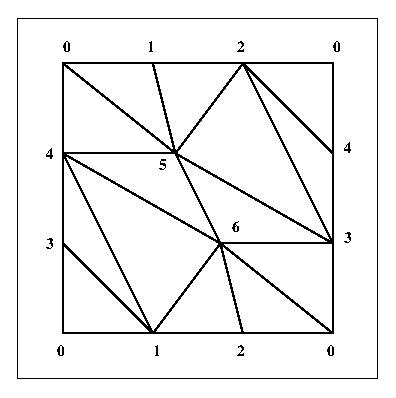
\includegraphics{torus2.eps}}
\vskip 0.40cm
%
The vertices will be named {\tt v0}, {\tt v1}, ..., {\tt v6}, {\tt v0} being the base point. The edges
will be named {\tt e01}, {\tt e02}, ...,  {\tt e56}, the list of faces of the edge $e_{ij}$ being
$(v_j\  v_i)$. The triangles will be named {\tt t013}, {\tt t015}, ..., {\tt t456}, the list of faces of
the triangle $t_{ijk}$ being $(e_{jk}\  e_{ik}\  e_{ij})$.
With this convention of describing the simplices, the call to {\tt build-finite-ss} is in simplified form:
{\footnotesize\begin{verbatim}
(setf torus2
    (build-finite-ss 
       '(v0  v1  v2  v3  v4  v5  v6 

         1 e01  (v1 v0)   e02  (v2 v0)   e03  (v3 v0)
           e04  (v4 v0)   e05  (v5 v0)   e06  (v6 v0)
           e12  (v2 v1)   e13  (v3 v1)   e14  (v4 v1)
           e15  (v5 v1)   e16  (v6 v1)   e23  (v3 v2)
           e24  (v4 v2)   e25  (v5 v2)   e26  (v6 v2)
           e34  (v4 v3)   e35  (v5 v3)   e36  (v6 v3)
           e45  (v5 v4)   e46  (v6 v4)   e56  (v6 v5)

         2 t013  (e13 e03 e01)  t015  (e15 e05 e01)  t024  (e24 e04 e02)
           t026  (e26 e06 e02)  t036  (e36 e06 e03)  t045  (e45 e05 e04)
           t125  (e25 e15 e12)  t126  (e26 e16 e12)  t134  (e34 e14 e13)
           t146  (e46 e16 e14)  t234  (e34 e24 e23)  t235  (e35 e25 e23)
           t356  (e56 e36 e35)  t456  (e56 e46 e45)  )))

Checking the 0-simplices...
Checking the 1-simplices...
Checking the 2-simplices...
[K1 Simplicial-Set]
\end{verbatim}}
After verification of the coherence of the description of the faces, the function
{\tt build-finite-ss} calls adequately the function {\tt build-smst} to create an instance
of the class {\tt SIMPLICIAL SET} subclass of the class {\tt CHAIN COMPLEX}. So that, it is easy for 
the user  to obtain the homology groups of the torus, for instance in dimension $1$:

{\footnotesize\begin{verbatim}
(chcm-homology  torus2 1)  ==>

Homology in dimension 1:

Component Z

Component Z
\end{verbatim}}
The function {\tt build-finite-ss} calls internally some verification functions mentioned above
to verify the coherence of the description of the simplicial set and gives 
an error message if the description of the simplicial set is incorrect. For instance:
{\footnotesize\begin{verbatim}
(setf mm (build-finite-ss 
   '(s0 s1 s2 s3 
     1 0-1 (s1 s0)  1-2 (s2 s1)  2-3 (s3 s2)
     2 0-1-2 (2-3 1-2 0-1))
  ))

Checking the 0-simplices...
Checking the 1-simplices...
Checking the 2-simplices...
Error: Noncoherent boundary operators detected by CHECK-FACES :
Simplex => <AbSm - 0-1-2>
del_0 o del_0 => <AbSm - S3>
del_0 o del_1 => <AbSm - S2>
\end{verbatim}}
\vskip 0.35cm
In the following examples, we show the power of {\tt build-finite-ss} for the description
of classical surfaces as simplicial sets, and in each case we  verify the well known 
homology groups of those surfaces. The examples of the torus
or the dunce-hat must be compared, as to the simplicity of the definition, to the respective 
ones in the previous page and in  the Homology chapter.
\newpage
%
\vskip 0.40cm
\centerline{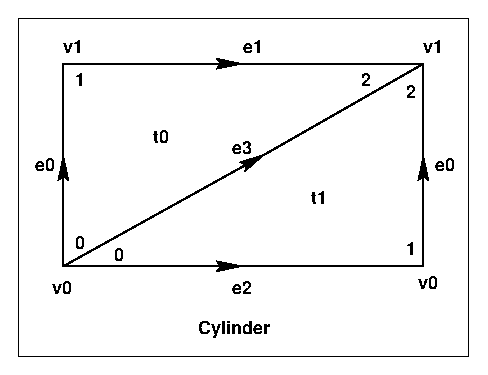
\includegraphics{cylinss.eps}}
\vskip 0.40cm
%

{\footnotesize\begin{verbatim}
(setf cylinss (build-finite-ss 
    '(v0 v1 
      1 e0 (v1 v0) e1 (v1 v1) e2 (v0 v0) e3 (v1 v0)
      2 t0 (e1 e3 e0) t1 (e0 e3 e2)) ))  ==>

[K2 Simplicial-Set]

(dotimes (i 3) (chcm-homology cylinss i)) ==>

Homology in dimension 0 :

Component Z

Homology in dimension 1 :

Component Z

Homology in dimension 2 :

---done---
\end{verbatim}}
\newpage
%
\vskip 0.40cm
\centerline{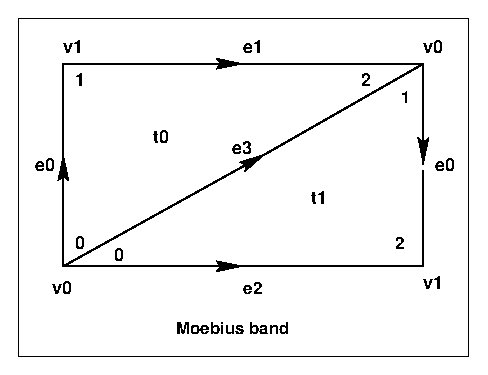
\includegraphics{moebiuss.eps}}
\vskip 0.40cm
%
{\footnotesize\begin{verbatim}
(setf moebiuss (build-finite-ss 
  '(v0 v1 
    1 e0 (v1 v0) e1 (v0 v1) e2 (v1 v0) e3 (v0 v0)
    2 t0 (e1 e3 e0) t1 (e0 e2 e3)) ))  ==>

[K3 Simplicial-Set]

(dotimes (i 3) (chcm-homology moebiuss i)) ==>

Homology in dimension 0 :

Component Z

Homology in dimension 1 :

Component Z

Homology in dimension 2 :

---done---
\end{verbatim}}
\newpage
%
\vskip 0.40cm
\centerline{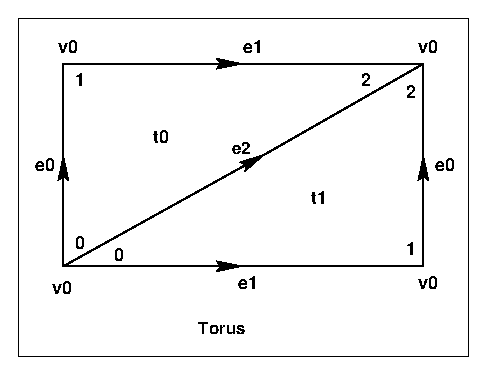
\includegraphics{toruss.eps}}
\vskip 0.40cm
%
{\footnotesize\begin{verbatim}
(setf toruss (build-finite-ss 
  '(v0
    1 e0 (v0 v0) e1 (v0 v0) e2 (v0 v0)
    2 t0 (e1 e2 e0) t1 (e0 e2 e1)) ))           ==>

[K4 Simplicial-Set]

(dotimes (i 3) (chcm-homology toruss i))  ==>

Homology in dimension 0 :

Component Z

Homology in dimension 1 :

Component Z

Component Z

Homology in dimension 2 :

Component Z

---done---
\end{verbatim}}
\newpage
%
\vskip 0.40cm
\centerline{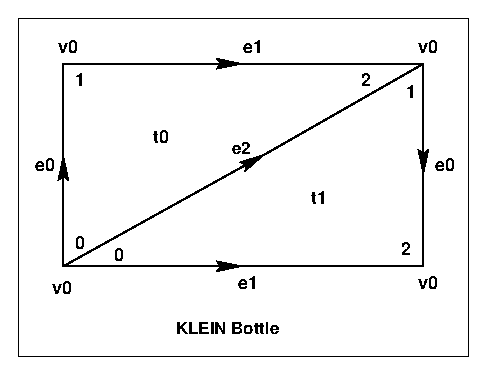
\includegraphics{bottless.eps}}
\vskip 0.40cm
%
{\footnotesize\begin{verbatim}
(setf bottless (build-finite-ss 
  '(v0
    1 e0 (v0 v0) e1 (v0 v0) e2 (v0 v0)
    2 t0 (e1 e2 e0) t1 (e0 e1 e2)) ))           ==>

[K5 Simplicial-Set]

(dotimes (i 3) (chcm-homology bottless i))  ==>

Homology in dimension 0 :

Component Z

Homology in dimension 1 :

Component Z/2Z

Component Z

Homology in dimension 2 :

---done---
\end{verbatim}}
\newpage
%
\vskip 0.40cm
\centerline{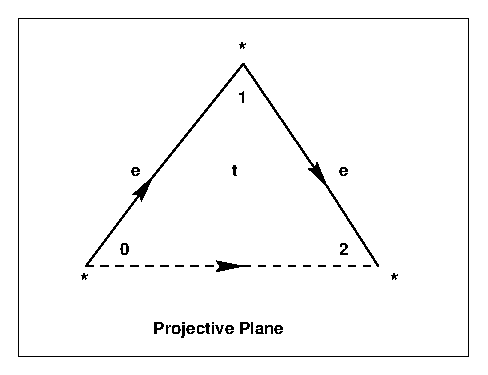
\includegraphics{ppss.eps}}
\vskip 0.40cm
%
{\footnotesize\begin{verbatim}
(setf ppss (build-finite-ss 
  '( *
     1 e (* *)
     2 t (e * e)) ))             ==>

[K6 Simplicial-Set]

(dotimes (i 3) (chcm-homology ppss i))  ==>

Homology in dimension 0 :

Component Z

Homology in dimension 1 :

Component Z/2Z

Homology in dimension 2 :

---done---
\end{verbatim}}
The user will note that the list of faces for the $2$--simplex {\tt t}, is
in simplified form. In particular, as the face $1$ of {\tt t} is the $0$--degeneracy
of the base point ``$*$'', it is sufficient to code the  face $1$ of {\tt t}
by ``{\tt *}'' instead of the complete form {\tt (0 *)}.
\newpage
%
\vskip 0.40cm
\centerline{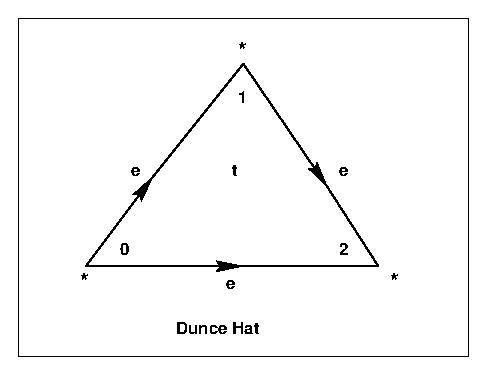
\includegraphics{duncess.eps}}
\vskip 0.40cm
%
{\footnotesize\begin{verbatim}
(setf duncess (build-finite-ss 
  '( *
     1 e (* *)
     2 t (e e e)) ))  ==>
 
[K7 Simplicial-Set]

(dotimes (i 3) (chcm-homology duncess i))  ==>

Homology in dimension 0 :

Component Z

Homology in dimension 1 :

Homology in dimension 2 :

---done---
\end{verbatim}}
\newpage

\section {Special simplicial sets}

The system provides useful functions to create interesting simplicial sets of constant usage.
In particular, the user is advised from now to use the following version of the standard
simplex implemented in {\tt Kenzo} and not the one given previously for simplicity reason. 

\subsection {The standard simplex}
{\parindent=0mm
{\leftskip=5mm 
{\tt delta} {\em dmns} \hfill {\em [Function]} \par}
{\leftskip=15mm 
Create\index{standard simplex} the standard simplex $\Delta^n$ with vertices $0,1,\ldots,n$,  
where {\em dmns} is the parameter for $n$.
This simplicial set is so important in the applications that
the implementor has decided to code the simplices in a  way similar to the coding\index{standard simplex!coding} 
of the degeneracy operators.
An {\bf increasing} sequence of non-negative integers describing a simplex, is coded
on a binary integer with the following convention: a number $i$ representing the vertex $i$ 
is the $(i+1)$--th binary bit of a machine word. The base point $0$ is the bit 1 in position 1 of the
word. This representation is very efficient for saving memory space but somehow awkward to read. \par}
{\leftskip=5mm 
{\tt delta-infinity} \hfill {\em [Function]} \par}
{\leftskip=15mm 
Create the locally effective standard simplex $\Delta^{\N}$ freely generated by the positive integers. \par}
{\leftskip=5mm 
{\tt deltab} \hfill {\em [Function]} \par}
{\leftskip=15mm 
Create the locally effective {\bf reduced} simplicial set $\bar \Delta$, built from
$\Delta^{\N}$ by identifying all the vertices to the base point. \par}
{\leftskip=5mm 
{\tt deltab2} \hfill {\em [Function]} \par}
{\leftskip=15mm 
Create the locally effective {\bf 1--reduced} simplicial set $\Delta_2^{\N}$, obtained from the above $\bar \Delta$,
by identification of all the edges with the base point. This is the efficient version of the coalgebra 
that is used as example in the cobar chapter. \par}
{\leftskip=5mm 
{\tt dlop-ext-int} {\em ext-dlop} \hfill {\em [Function]}\par}
{\leftskip=15mm 
Code on an integer the valid list (increasing order) representing the simplex {\em ext-dlop} of the
standard simplex. \par}
{\leftskip=5mm 
{\tt dlop-int-ext} {\em dgop} \hfill {\em [Function]}\par}
{\leftskip=15mm 
Give the list representing a simplex of the standard simplex from the integer {\em dgop}. \par}
}
\newpage
{\parindent=0mm
{\leftskip=5mm 
{\tt vertex-i} {\em absm i} \hfill {\em [Function]}\par}
{\leftskip=15mm 
Give the $i$--th vertex of the (coded, degenerate or not) abstract simplex {\em absm} belonging to a simplicial set
of the $\Delta$ family. \par}
{\leftskip=5mm 
{\tt absm-ext-int} {\em vlist} \hfill {\em [Function]}\par}
{\leftskip=15mm 
Create a valid abstract simplex of the $\Delta$ family from the simplex {\em vlist} written as a non-decreasing list of 
non--negative integers (i.e coding of any degenerate or non--degenerate simplex of the $\Delta$ fa\-mi\-ly). \par}
{\leftskip=5mm 
{\tt absm-int-ext} {\em absm} \hfill {\em [Function]}\par}
{\leftskip=15mm 
From an internal coded form of an abstract simplex of the $\Delta$ family, create the  non-decreasing list
of non--negative integers representing the canonical external form of such a simplex. \par}
{\leftskip=5mm 
{\tt soft-delta} {\em dmns} \hfill {\em [Function]} \par}
{\leftskip=15mm 
Create another version of the standard simplex $\Delta^n$ designed for a better clarity in
the printing of the results at testing time. More precisely, the simplices are represented internally by a list
of the form {\tt (:delt {\em binary-code})}. With this representation, the system is able to
recognize a coded simplex and to print it in a readable form. For the user, the only
requirement is to write a simplex coded $n$ as {\tt (d {\em n})}, where {\tt d} is the macro
building the internal representation (see the examples). Attention: the above conversion
functions do not work with this representation. \par}
{\leftskip=5mm 
{\tt soft-delta-infinity} \hfill {\em [Function]} \par}
{\leftskip=15mm 
Create another version of the locally effective standard simplex $\Delta^{\N}$ 
(see the function {\tt soft-delta} above). \par}
}

\subsection* {Examples}

{\footnotesize\begin{verbatim}
(setf d3 (delta 3))  ==>

[K8 Simplicial-Set]
\end{verbatim}}
The simplices $2$, $4$ and  $8$ are the coded representation of the vertices $1$, $2$ and $3$:
{\footnotesize\begin{verbatim}
(cmpr d3 2 4)  ==>

:LESS

(cmpr d3 4 4)  ==>

:EQUAL

(cmpr d3 8 4)  ==>

:GREATER
\end{verbatim}}
The list returned by the following statement  getting the basis of $\Delta^3$ in 
dimension $2$, namely {\tt (7 11 13 14)} is in fact the coded list 
of the following simplices {\tt ((0 1 2) (0 1 3) (0 2 3) (1 2 3))}. 
{\footnotesize\begin{verbatim}
(basis d3 2)  ==>

(7 11 13 14)
\end{verbatim}}
In the following statement, 
the integer $21$ represents the simplex in dimension $2$, {\tt (0 1 4)}, $1$ represents the operator $\partial_1$
and the face is therefore {\tt (0 4)} represented as the integer $17$. 
{\footnotesize\begin{verbatim}
(face d3 1 2 21)  ==>

<AbSm - 17>
\end{verbatim}}
We may obtain the same result, using:
{\footnotesize\begin{verbatim}
(face d3 1 2 (dlop-ext-int '(0 1 4)))  ==>

<AbSm - 17>
\end{verbatim}}
Let us test the conversion functions.
{\footnotesize\begin{verbatim}
(vertex-i (absm 0 1) 0)  ==>

0

(vertex-i (absm 1 1) 0)  ==>

0

(vertex-i (absm 1 1) 1)  ==>

0

(vertex-i (absm 0 7) 2)  ==>

2

(absm-ext-int '(0 0 0 1 2 3 3 3))  ==>

<AbSm 6-5-1-0 15>

(absm-ext-int '(0 1 1 1 2))  ==>

<AbSm 2-1 7>

(absm-int-ext (absm-ext-int '(0 0 0 1 2 3 3 3)))  ==>

(0 0 0 1 2 3 3 3)
\end{verbatim}}
The following  call to the macro {\tt ?} returns the boundary of the simplex {\tt (0 2 3)}
of $\Delta^3$, the integers $5$, $9$ and $12$ representing respectively the simplices
{\tt (0 2)}, {\tt (0 3)} and {\tt (2 3)}. The application of the coproduct {\tt dgnl} to the
simplex {\tt (0 1 2 3)}, coded $15$, is also easily interpreted:
{\footnotesize\begin{verbatim}
(? d3 2 13)

-----------------------------------------------------------------------{CMB 1}
<1 * 5>
<-1 * 9>
<1 * 12>
------------------------------------------------------------------------------

(dgnl d3 3 15)  ==>

----------------------------------------------------------------------{CMBN 3}
<1 * <TnPr 1 15>>
<1 * <TnPr 3 14>>
<1 * <TnPr 7 12>>
<1 * <TnPr 15 8>>
------------------------------------------------------------------------------
\end{verbatim}}
We may show now some examples with the {\it soft} version of the standard
simplex. Using the macro {\tt d} and the function {\tt dlop-ext-int} the user may work
with a readable form of the simplices and the degeneracy operators.
{\footnotesize\begin{verbatim}
(setf d3 (soft-delta 3))  ==>

[K10 Simplicial-Set]

(cmpr d3 (d 2) (d 4))  ==>

:LESS

(basis d3 1)  ==>

(0-1 0-2 1-2 0-3 1-3 2-3)
\end{verbatim}}
\newpage
{\footnotesize\begin{verbatim}
(dgnl d3 3 (d (dlop-ext-int '(0 1 2 3))))  ==>

----------------------------------------------------------------------{CMBN 3}
<1 * <TnPr 0 0-1-2-3>>
<1 * <TnPr 0-1 1-2-3>>
<1 * <TnPr 0-1-2 2-3>>
<1 * <TnPr 0-1-2-3 3>>
------------------------------------------------------------------------------

(face d3 1 2 (d (dlop-ext-int '(0 2 4))))  ==>

<AbSm - 0-4>

(? d3 2 (d (dlop-ext-int '(0 2 3))))  ==>

----------------------------------------------------------------------{CMBN 1}
<1 * 0-2>
<-1 * 0-3>
<1 * 2-3>
------------------------------------------------------------------------------
\end{verbatim}}
\newpage

\subsection {Spheres, Moore spaces and projectives spaces}
{\parindent=0mm
{\leftskip=5mm 
{\tt sphere} {\em n} \hfill {\em [Function]} \par}
{\leftskip=15mm 
Create\index{sphere} a simplicial set, a model  for the sphere of dimension $n$, ($n \geq 0$). 
This is a typical example where the differential is known a priori to be null, so the {\tt :intr-bndr}
keyword parameter is set to function {\tt zero-pure-dffr}.
This function generates a name {\tt S{\em n}} for the {\bf unique} simplex of dimension $n$
whose faces are the degeneracies of the base point labelled ``{\tt *}''.  \par}  
{\leftskip=5mm 
{\tt sphere-wedge} {\em dmns1 ... dmnsn} \hfill {\em [Function]} \par}
{\leftskip=15mm 
Create\index{sphere!wedge} a simplicial set for the wedge of spheres. Here, the $dmns_i$ are integers,
namely the dimensions of the spheres to be wedged. The differential is null.
In the  representation created by the software, the $0$--simplex (base point) is labelled
``{\tt *}'' and in dimension $p$ the simplexes are labelled {\tt S{\em p}-{\em 1}}, ..., 
{\tt S{\em p}-{\em s}},  where
{\em s} is the number of spheres of dimension $p$ in the wedge. (See the example). \par}
{\leftskip=5mm 
{\tt moore} {\em  p n} \hfill {\em [Function]}\par}
{\leftskip=15mm 
Construct\index{Moore space} a simplicial set, a model for  ${\rm Moore}({\Z}/{p{\Z}},n)$. 
The integers $p$ and $n$ must satisfy  the conditions $p>1,\ n> 2p-4$, otherwise
the result is undefined. 
${\rm Moore}({\Z}/{p{\Z}},n)$ is a space, whose the only non--null homology groups are $H_0={\Z}$
and $H_n={\Z}/{p{\Z}}$. A Moore space has only three non--degenerate simplices, namely in dimension
$0$, $n$ and $n+1$. A number $p$ of faces of the  $(n+1)$--simplex are identified with the $n$--simplex, 
the others faces being contracted on the base point.
In the  representation created by the software, the $0$--simplex (base point),
the $n$--simplex and the $(n+1)$--simplex are respectively labelled
``{\tt *}'', {\tt M{$n$}} and {\tt N{$n'$}}, where $n'=n+1$. \par}
{\leftskip=5mm 
{\tt R-proj-space \&optional} {\em k l} \hfill {\em [Function]} \par}
{\leftskip=15mm 
If $k=1$ or omitted, build a simplicial set model\index{projective spaces} of $K({\Z}_2,1)= P^\infty {\R}$. 
In dimension $n$, this simplicial set has only one non-degenerate simplex, namely the integer $n$. 
The faces of this non-degenerate simplex $n$ are given by the following formulas:
$\partial_0 n = \partial_n n = n-1$ and for $i \not= 0$ and $i \not=n$,  $\partial_i n= \eta_{i-1} (n-2)$.  
If $k >1$, build an 
analogous simplicial set but with no simplices in dimensions $1 \leq m < k$. If in addition to $k$ 
the argument $l$, ($l \geq k$), is provided, build
an analogous simplicial set but with no simplices in dimensions $m \geq l$. \par 
}

\subsection*{Examples}

Let us define first, an auxiliary function {\tt show-structure}\index{function {\tt show-structure}} 
with $2$ arguments {\em ss} and {\em dmn},
to show the structure (i.e. generators and faces) of the simplicial set  {\em ss},  
from the dimension $0$ up to the dimension {\em dmn} included.
{\footnotesize\begin{verbatim}
(defun show-structure (ss dmn)
 (dotimes (i (1+ dmn))
   (format t "~2%Dimension = ~D :" i)
   (case i
     (0 (format t "~2%~8TVertices : ~8T~A" (basis ss 0)))
     (otherwise
        (dolist (s (basis ss i))
            (format t "~2%~8TSimplex : ~A~2%~16TFaces : ~A"
                    s (mapcar #'(lambda (j) (face ss j i s))
                                (<a-b> 0 i)))))
  )))
\end{verbatim}}
In these elementary examples, we show the structure of some simplicial sets built
from the functions above. Let us begin with $S^2$.

{\footnotesize\begin{verbatim}
(setf s2 (sphere 2))  ==>

[K11 Simplicial-Set]

(bspn s2)  ==>

*
\end{verbatim}}
Applying the function {\tt basis}, we see that the only non-null simplices are in dimension $0$
and $2$.
{\footnotesize\begin{verbatim}
(dotimes (i 4) (print (basis s2 i)))  ==>

(*) 
NIL 
(S2) 
NIL 
\end{verbatim}}
In dimension $2$, the $3$ faces of the simplicial set are all the degeneracy $\eta_0$ 
of the base point.
{\footnotesize\begin{verbatim}
(mapcar #'(lambda(i)(face s2 i 2 's2)) '(0 1 2))  ==>

(<AbSm 0 *> <AbSm 0 *> <AbSm 0 *>)

(face s2 5 7 (absm (dgop-ext-int '(5 3 1 0)) 's2))  ==>

<AbSm 3-1-0 S2>

(face s2 2 7 (absm (dgop-ext-int '(5 3 1 0)) 's2))  ==>

<AbSm 4-2-0 S2>
\end{verbatim}}
The differential of the simplex {\tt s2} in dimension $2$ is of course the null combination
of degree $1$:
{\footnotesize\begin{verbatim}
(? s2 2 's2)  ==>

-----------------------------------------------------------------------{CMB 1}
------------------------------------------------------------------------------

\end{verbatim}}

Now, let us see the stucture of $S^3$, using our auxiliary function {\tt show-structure}.
{\footnotesize\begin{verbatim}
(setf s3 (sphere 3))  ==>

[K12 Simplicial-Set]

(show-structure s3 3)  ==>

Dimension = 0 :

        Vertices :  (*)

Dimension = 1 :

Dimension = 2 :

Dimension = 3 :

        Simplex : S3

                Faces : (<AbSm 1-0 *> <AbSm 1-0 *> <AbSm 1-0 *> <AbSm 1-0 *>)
\end{verbatim}}

The space ${\rm Moore}(2,1)$ is the projective plane:
{\footnotesize\begin{verbatim}

(setf p2 (moore 2 1))  ==>

[K13 Simplicial-Set]

(show-structure p2 2)  ==>

Dimension = 0 :

        Vertices :  (*)

Dimension = 1 :

        Simplex : M1

                Faces : (<AbSm - *> <AbSm - *>)

Dimension = 2 :

        Simplex : N2

                Faces : (<AbSm - M1> <AbSm 0 *> <AbSm - M1>)
\end{verbatim}}
In the following example, note the identification of $p$ faces 
of the $(n+1)$--simplex with the $n$--simplex.
{\footnotesize\begin{verbatim}
(setf sp2r (moore 2 2))  ==>

[K15 Simplicial-Set]

(show-structure sp2r 3)  ==>

Dimension = 0 :

        Vertices :  (*)

Dimension = 1 :

Dimension = 2 :

        Simplex : M2

                Faces : (<AbSm 0 *> <AbSm 0 *> <AbSm 0 *>)

Dimension = 3 :

        Simplex : N3

                Faces : (<AbSm - M2> <AbSm 1-0 *> <AbSm - M2>
                         <AbSm 1-0 *>)

\end{verbatim}}
Let us see an example of a wedge of spheres:
{\footnotesize\begin{verbatim}
(setf w (sphere-wedge 3 2 3))  ==>

[K16 Simplicial-Set]

(show-structure w 5)  ==>

Dimension = 0 :

        Vertices :  (*)

Dimension = 1 :

Dimension = 2 :

        Simplex : S2-1

                Faces : (<AbSm 0 *> <AbSm 0 *> <AbSm 0 *>)

Dimension = 3 :

        Simplex : S3-1

                Faces : (<AbSm 1-0 *> <AbSm 1-0 *> <AbSm 1-0 *>
                         <AbSm 1-0 *>)

        Simplex : S3-2

                Faces : (<AbSm 1-0 *> <AbSm 1-0 *> <AbSm 1-0 *>
                         <AbSm 1-0 *>)

Dimension = 4 :

Dimension = 5 :

(cmpr w 's3-1 's3-2)  ==>

:LESS

(face w 2 3 's3-1)  ==>

<AbSm 1-0 *>

(? w 3 's3-2)  ==>

-----------------------------------------------------------------------{CMB 2}
------------------------------------------------------------------------------
\end{verbatim}}
\newpage
Let us show now some examples with the simplicial sets generated by the
function {\tt R-proj-space}.
{\footnotesize\begin{verbatim}
(setf p1 (R-proj-space))  ==>

[K20 Simplicial-Set]

(dotimes (i 7)(print(basis p1 i)))  ==>

(0) 
(1) 
(2) 
(3) 
(4) 
(5) 
(6) 

(show-structure p1 5)  ==>

Dimension = 0 :

        Vertices :  (0)

Dimension = 1 :

        Simplex : 1

                Faces : (<AbSm - 0> <AbSm - 0>)

Dimension = 2 :

        Simplex : 2

                Faces : (<AbSm - 1> <AbSm 0 0> <AbSm - 1>)

Dimension = 3 :

        Simplex : 3

                Faces : (<AbSm - 2> <AbSm 0 1> <AbSm 1 1> <AbSm - 2>)

Dimension = 4 :

        Simplex : 4

                Faces : (<AbSm - 3> <AbSm 0 2> <AbSm 1 2> <AbSm 2 2> <AbSm - 3>)

Dimension = 5 :

        Simplex : 5

                Faces : (<AbSm - 4> <AbSm 0 3> <AbSm 1 3> <AbSm 2 3> <AbSm 3 3> 
                         <AbSm - 4>)

(dotimes (i 5)(chcm-homology p1 i)) ==>

Homology in dimension 0 :

Component Z

Homology in dimension 1 :

Component Z/2Z

Homology in dimension 2 :

---done---

Homology in dimension 3 :

Component Z/2Z

Homology in dimension 4 :

---done---

(setf p2 (R-proj-space 2))  ==>

[K21 Simplicial-Set]

(show-structure p2 5)  ==>

Dimension = 0 :

        Vertices :  (0)

Dimension = 1 :

Dimension = 2 :

        Simplex : 2

                Faces : (<AbSm 0 0> <AbSm 0 0> <AbSm 0 0>)

Dimension = 3 :

        Simplex : 3

                Faces : (<AbSm - 2> <AbSm 1-0 0> <AbSm 1-0 0> <AbSm - 2>)

Dimension = 4 :

        Simplex : 4

                Faces : (<AbSm - 3> <AbSm 0 2> <AbSm 1 2> <AbSm 2 2> <AbSm - 3>)

Dimension = 5 :

        Simplex : 5

                Faces : (<AbSm - 4> <AbSm 0 3> <AbSm 1 3> <AbSm 2 3> <AbSm 3 3> 
                         <AbSm - 4>)

(dotimes (i 5)(chcm-homology p2 i))  ==>

Homology in dimension 0 :

Component Z

Homology in dimension 1 :

---done---

Homology in dimension 2 :

Component Z

Homology in dimension 3 :

Component Z/2Z

Homology in dimension 4 :

---done---

(setf pr3 (R-proj-space 3))  ==>

[K22 Simplicial-Set]

(show-structure pr3 4)  ==>

Dimension = 0 :

        Vertices :  (0)

Dimension = 1 :

Dimension = 2 :

Dimension = 3 :

        Simplex : 3

                Faces : (<AbSm 1-0 0> <AbSm 1-0 0> <AbSm 1-0 0> <AbSm 1-0 0>)

Dimension = 4 :

        Simplex : 4

                Faces : (<AbSm - 3> <AbSm 2-1-0 0> <AbSm 2-1-0 0> 
                         <AbSm 2-1-0 0> <AbSm - 3>)

(dotimes (i 7)  (print (? pr3 i i)))  ==>

----------------------------------------------------------------------{CMBN -1}
------------------------------------------------------------------------------

----------------------------------------------------------------------{CMBN 0}
------------------------------------------------------------------------------

----------------------------------------------------------------------{CMBN 1}
------------------------------------------------------------------------------

----------------------------------------------------------------------{CMBN 2}
------------------------------------------------------------------------------

----------------------------------------------------------------------{CMBN 3}
<2 * 3>
------------------------------------------------------------------------------

----------------------------------------------------------------------{CMBN 4}
------------------------------------------------------------------------------

----------------------------------------------------------------------{CMBN 5}
<2 * 5>
------------------------------------------------------------------------------
\end{verbatim}}
Let us use now the parameter {\em l}, allowing the truncation in the upper dimensions.
{\footnotesize\begin{verbatim}
(setf p12 (R-proj-space 1 2))  ==>

[K23 Simplicial-Set]

(show-structure p12 2)  ==>

Dimension = 0 :

        Vertices :  (0)

Dimension = 1 :

        Simplex : 1

                Faces : (<AbSm - 0> <AbSm - 0>)

Dimension = 2 :
\end{verbatim}}
Setting $k=l$ does not creates something amazing!
{\footnotesize\begin{verbatim}
(setf p22 (R-proj-space 2 2))  ==>

[K28 Simplicial-Set]

(show-structure p22 2)  ==>

Dimension = 0 :

        Vertices :  (0)

Dimension = 1 :

Dimension = 2 :

(setf p47 (R-proj-space 4 7))  ==>

[K33 Simplicial-Set]

(show-structure p47 8)  ==>

Dimension = 0 :

        Vertices :  (0)

Dimension = 1 :

Dimension = 2 :

Dimension = 3 :

Dimension = 4 :

        Simplex : 4

                Faces : (<AbSm 2-1-0 0> <AbSm 2-1-0 0> <AbSm 2-1-0 0> 
                         <AbSm 2-1-0 0> <AbSm 2-1-0 0>)

Dimension = 5 :

        Simplex : 5

                Faces : (<AbSm - 4> <AbSm 3-2-1-0 0> <AbSm 3-2-1-0 0> 
                         <AbSm 3-2-1-0 0> <AbSm 3-2-1-0 0> <AbSm - 4>)

Dimension = 6 :

        Simplex : 6

                Faces : (<AbSm - 5> <AbSm 0 4> <AbSm 1 4> <AbSm 2 4> 
                         <AbSm 3 4> <AbSm 4 4> <AbSm - 5>)

Dimension = 7 :

Dimension = 8 :
\end{verbatim}}

\newpage

\section {Cartesian product of  simplicials sets }

Let $X$ and $Y$ be two simplicial\index{simplicial sets!cartesian product}
sets, the construction of $X\times Y$ is based on the very definition $(X\times Y)_n =X_n\times Y_n$
where $X_n$, $Y_n$ and $(X\times Y)_n$ are the {\em possibly degenerate} simplices of $X$, $Y$ and $X\times Y$
respectively. A simplex of the product $X\times Y$ is characterized  by its projections on the factors $X$ and $Y$.
\par
The {\em non--degenerate} simplices of $X\times Y$  are
represented internally in the system by a lisp object of the form:
\begin{center}
{\tt (:crpr ({\em dgop1}.{\em gmsm1}).({\em dgop2}.{\em gmsm2}))}
\end{center}
where,
\begin{enumerate}
\item {\tt dgop1} is an integer representing a coded degeneracy operator.
\item {\tt gmsm1} is a non-degenerate simplex of $X$, to which is applied the degeneracy operator
{\tt dgop1}.
\item {\tt dgop2} is an integer representing a coded degeneracy operator.
\item {\tt gmsm2} is a non-degenerate simplex of $Y$, to which is applied the degeneracy operator
{\tt dgop2}.
\end{enumerate}
This object must be a {\em non--degenerate} simplex of $X \times Y$,
that is to say, the degeneracy operators {\tt dgop1} and {\tt dgop2} must not have a common $\eta_j$, and 
therefore their list representations must have a void intersection.
The coded representation by  binary bit positions, has the same property. The corresponding type
is {\tt CRPR}.
To construct such an object, one may use the macro {\tt crpr}. As usual, a printing method
has been defined to reflect the structure of the product under the form:
\begin{center}
{\tt <CrPr {\em ext-dgop1 gmsm1 ext-dgop2 gmsm2}> }
\end{center}
where  the sequence of the operators $\eta_i$ is printed in explicit form (this is the meaning of {\em ext-dgop}).
If this sequence of $\eta_i$  is void, i.e. if the simplex {\em gmsm} is not degenerate, 
the symbol {\tt -} is printed instead.
\newpage

\subsection {Functions and macros for the product of simplicial sets}

{\parindent=0mm
{\leftskip=5mm 
{\tt crpr} {\em dgop1 gmsm1 dgop2 gmsm2} \hfill {\em [Macro]} \par}
{\leftskip=15mm 
Build an object of type {\tt CRPR}, using directly the integer coding for the
degeneracy operators. The arguments {\em gmsm1} and {\em gmsm2} are non-degenerate
simplices.  \par}
{\leftskip=5mm 
{\tt crpr} {\em absm1 absm2} \hfill {\em [Macro]} \par}
{\leftskip=15mm 
Build an object of type {\tt CRPR}, using two abstract simplices {\em absm1} and {\em absm2}. If these
abstract simplices are degenerate, the de\-ge\-ne\-ra\-cy operators must verify the condition of
the definition, i.e. no common $\eta_i$. \par}
{\leftskip=5mm 
{\tt 2absm-acrpr} {\em absm1 absm2} \hfill {\em [Function]} \par}
{\leftskip=15mm 
Build an abstract simplex, i.e. object of type {\tt ABSM}, cartesian pro\-duct of both abstract simplices {\em absm1} 
and {\em absm2}. In contrast with the previous function, there is no condition upon the
de\-ge\-ne\-ra\-cy operators of the abstract simplices. Of course, the function {\tt 2absm-acrpr} returns
a legal abstract simplex. \par}
{\leftskip=5mm 
{\tt crpr-p} {\em object} \hfill {\em [Predicate]} \par}
{\leftskip=15mm 
Test if {\em object} is of type {\tt CRPR}. \par}
{\leftskip=5mm 
{\tt dgop1} {\em crpr} \hfill {\em [Macro]} \par}
{\leftskip=15mm 
Select the degeneracy operator {\em dgop1} from the object {\tt crpr}. \par}
{\leftskip=5mm 
{\tt gmsm1} {\em crpr} \hfill {\em [Macro]} \par}
{\leftskip=15mm 
Select the geometric simplex {\em gmsm1} from the object {\tt crpr}. \par}
{\leftskip=5mm 
{\tt dgop2} {\em crpr} \hfill {\em [Macro]} \par}
{\leftskip=15mm 
Select the degeneracy operator {\em dgop2} from the object {\tt crpr}. \par}
{\leftskip=5mm 
{\tt gmsm2} {\em crpr} \hfill {\em [Macro]} \par}
{\leftskip=15mm 
Select the geometric simplex {\em gmsm2} from the object {\tt crpr}. \par}
{\leftskip=5mm 
{\tt absm1} {\em crpr} \hfill {\em [Macro]} \par}
{\leftskip=15mm 
Build the abstract simplex {\tt (absm {\em dgop1 gmsm1})} from {\em crpr}. \par}
{\leftskip=5mm 
{\tt absm2} {\em crpr} \hfill {\em [Macro]} \par}
{\leftskip=15mm 
Build the abstract simplex {\tt (absm {\em dgop2 gmsm2})} from {\em crpr}. \par}
{\leftskip=5mm 
{\tt crts-prdc} {\em smst1 smst2} \hfill {\em [Function]} \par}
{\leftskip=15mm 
Build the simplicial set, cartesian product $smst1 \times smts2$. \par}
}

\subsection* {Examples}

In the first example, note that the coded representations of $\eta_1$ and $\eta_2$ are
respectively $2$ and $4$, but these degeneracy operators appear clearly as $1$ and $2$ in the printed result.
In the second statement, the integer $28$ is the coded representation of the degeneracy {\tt (4 3 2)}.
{\footnotesize\begin{verbatim}
(crpr 2 'a 4 'b)  ==>

<CrPr 1 A 2 B>

(crpr 0 '(0 1 2 3 4 5) 28 '(0 1 2))   ==>

<CrPr - (0 1 2 3 4 5) 4-3-2 (0 1 2)>
\end{verbatim}}
For more clarity, one may also write:
{\footnotesize\begin{verbatim}
(crpr 0 '(0 1 2 3 4 5) (dgop-ext-int '(4 3 2)) '(0 1 2))   ==>

<CrPr - (0 1 2 3 4 5) 4-3-2 (0 1 2)>
\end{verbatim}}
In the following example, we see that both functions {\tt crpr} and
{\tt 2absm-acrpr} return the same geometric simplex,
{\footnotesize\begin{verbatim}
(crpr (absm 4 'a)(absm 3 'b))  ==>

<CrPr 2 A 1-0 B>

(2absm-acrpr (absm 4 'a)(absm 3 'b))  ==>

<AbSm - <CrPr 2 A 1-0 B>>
\end{verbatim}}
whereas, in the following call to {\tt crpr}, the condition upon the degeneracy
operator is not respected and the result is an illegal cartesian product.
The function {\tt 2absm-acrpr} returns the correct answer.
{\footnotesize\begin{verbatim}
(crpr (absm 5 'a)(absm 3 'b))  ==>

<CrPr 2-0 A 1-0 B>     ;;; ILLEGAL!

(2absm-acrpr (absm 5 'a) (absm 3 'b))  ==>

<AbSm 0 <CrPr 1 A 0 B>>
\end{verbatim}}
The following example is particularly instructive. The simplicial set
whose the realization is homeomorphic to the  square is built by using the product of two segments.
A call like {\tt (delta n)} builds  the standard $n$--simplex. So first, we generate
two copies {\tt X} and {\tt Y} of the standard $1$--simplex and we list the abstract simplices 
up to dimension $2$ for a better understanding of the components of the product {\tt XY}.
{\footnotesize\begin{verbatim}
(setf X (delta 1))  ==>

[K4 Simplicial-Set]

(setf Y X)  ==>

[K4 Simplicial-Set]
\end{verbatim}}
%
\vskip 0.40cm
\centerline{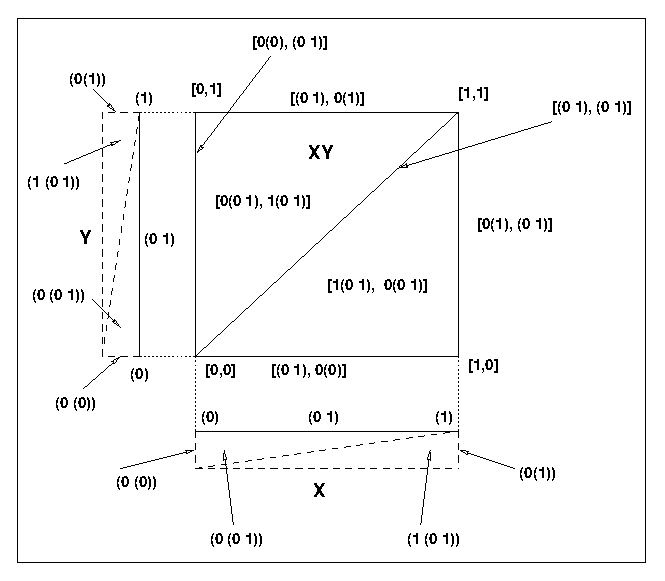
\includegraphics{ssquare.eps}}
\vskip 0.40cm
%

In list representation (non-coded simplices), the  abstract simplices of $X$ up to the dimension $2$, 
including the degenerate ones are:
\begin{itemize}
\item {Dimension 0}: {\footnotesize {\tt <AbSm - (0)>, <AbSm - (1)>}}. 
\item {Dimension 1}: {\footnotesize {\tt <AbSm 0 (0)>,  <AbSm 0 (1)>,  <AbSm - (0 1)>}}. 
\item {Dimension 2}: {\footnotesize {\tt <AbSm 1-0 (0)>, <AbSm 1-0 (1)>,  <AbSm 0 (0 1)>, \par
 <AbSm 1 (0 1)>}}.
\end{itemize}

Let us look first at the non-degenerate simplices of the simplicial set $X \times Y$. Those simplices are objects
of type  {\tt CRPR}. In dimension $1$, we see that some projections are
degeneracies of vertices and, in dimension $2$, the projections are all degeneracies of
the $1$--simplex {\tt(0 1)} coded as $3$. Nevertheless, all the listed simplices are {\em geometric} 
simplices (i.e. non-degenerate ones) of the product {\tt XY}. The diagram above shows the relationship between
the $3$ simplicial sets. 
{\footnotesize\begin{verbatim}
(setf XY (crts-prdc X Y))  ==>

[K5 Simplicial-Set]

(show-structure XY 2)  ==>

Dimension = 0 :

        Vertices :  (<CrPr - 1 - 1> <CrPr - 1 - 2> <CrPr - 2 - 1>
                     <CrPr - 2 - 2>)

Dimension = 1 :

        Simplex : <CrPr - 3 - 3>

                Faces : (<AbSm - <CrPr - 2 - 2>>
                         <AbSm - <CrPr - 1 - 1>>)

        Simplex : <CrPr - 3 0 1>

                Faces : (<AbSm - <CrPr - 2 - 1>>
                         <AbSm - <CrPr - 1 - 1>>)

        Simplex : <CrPr - 3 0 2>

                Faces : (<AbSm - <CrPr - 2 - 2>>
                         <AbSm - <CrPr - 1 - 2>>)

        Simplex : <CrPr 0 1 - 3>

                Faces : (<AbSm - <CrPr - 1 - 2>>
                         <AbSm - <CrPr - 1 - 1>>)

        Simplex : <CrPr 0 2 - 3>

                Faces : (<AbSm - <CrPr - 2 - 2>>
                         <AbSm - <CrPr - 2 - 1>>)

Dimension = 2 :

        Simplex : <CrPr 0 3 1 3>

                Faces : (<AbSm - <CrPr - 3 0 2>>
                         <AbSm - <CrPr - 3 - 3>>
                         <AbSm - <CrPr 0 1 - 3>>)

        Simplex : <CrPr 1 3 0 3>

                Faces : (<AbSm - <CrPr 0 2 - 3>>
                         <AbSm - <CrPr - 3 - 3>>
                         <AbSm - <CrPr - 3 0 1>>)
\end{verbatim}}
To be more readable we may translate the coded representations of the de\-ge\-ne\-ra\-cy operators
and of the simplices in the list representation:
{\footnotesize\begin{verbatim}

Dimension 0 :

        Vertices : (<CrPr - (0) - (0)> 
                    <CrPr - (0) - (1)> 
                    <CrPr - (1) - (0)> 
                    <CrPr - (1) - (1)>)

Dimension 1 :

        Simplex : <CrPr 0 (0) - (0 1)>

                Faces : (<AbSm - <CrPr - (0) - (1)> >
                         <AbSm - <CrPr - (0) - (0)> >)

        Simplex : <CrPr 0 (1) - (0 1)>

                Faces : (<AbSm - <CrPr - (1) - (1)> >
                         <AbSm - <CrPr - (1) - (0)> >)

        Simplex : <CrPr - (0 1) 0 (0)>

                Faces : (<AbSm - <CrPr - (1) - (0)> >
                         <AbSm - <CrPr - (0) - (0)> >)

        Simplex : <CrPr - (0 1) 0 (1)>

                Faces : (<AbSm - <CrPr - (1) - (1)> >
                         <AbSm - <CrPr - (0) - (1)> >)

        Simplex : <CrPr - (0 1) - (0 1)>

                Faces : (<AbSm - <CrPr - (1) - (1)> >
                         <AbSm - <CrPr - (0) - (0)> >)

Dimension 2 :

        Simplex : <CrPr 0 (0 1) 1 (0 1)>

                Faces : (<AbSm - <CrPr - (0 1) 0 (1)> >
                         <AbSm - <CrPr - (0 1) - (0 1)> >
                         <AbSm - <CrPr 0 (0) - (0 1)> >)

        Simplex : <CrPr 1 (0 1) 0 (0 1)>

                Faces : (<AbSm - <CrPr 0 (1) - (0 1)> >
                         <AbSm - <CrPr - (0 1) - (0 1)> >
                         <AbSm - <CrPr - (0 1) 0 (0)> >)
\end{verbatim}}
In an analogous way, let us build the torus as the cartesian product
of two $1$--spheres. We recall that the base point of the sphere is named {\tt *}.
{\footnotesize\begin{verbatim}
(setf s1xs1 (crts-prdc (sphere 1) (sphere 1)))  ==>

[K15 Simplicial-Set]

(show-structure s1xs1 2)  ==>

Dimension = 0 :

        Vertices :  (<CrPr - * - *>)

Dimension = 1 :

        Simplex : <CrPr - S1 - S1>

                Faces : (<AbSm - <CrPr - * - *>>
                         <AbSm - <CrPr - * - *>>)

        Simplex : <CrPr - S1 0 *>

                Faces : (<AbSm - <CrPr - * - *>>
                         <AbSm - <CrPr - * - *>>)

        Simplex : <CrPr 0 * - S1>

                Faces : (<AbSm - <CrPr - * - *>>
                         <AbSm - <CrPr - * - *>>)

Dimension = 2 :

        Simplex : <CrPr 0 S1 1 S1>

                Faces : (<AbSm - <CrPr - S1 0 *>>
                         <AbSm - <CrPr - S1 - S1>>
                         <AbSm - <CrPr 0 * - S1>>)

        Simplex : <CrPr 1 S1 0 S1>

                Faces : (<AbSm - <CrPr 0 * - S1>>
                         <AbSm - <CrPr - S1 - S1>>
                         <AbSm - <CrPr - S1 0 *>>)
\end{verbatim}}
Let us verify that  $S^1\times S^1$ has  the same  homology groups as the torus.
{\footnotesize\begin{verbatim}
(dotimes (i 3)(chcm-homology s1xs1 i)) ==>
  
Homology in dimension 0 :

 Component Z

Homology in dimension 1 :

 Component Z

 Component Z

Homology in dimension 2 :

 Component Z

\end{verbatim}}
Of course, we may generate more complex products, whose basis are composed of rather long
lists of simplices as shown below. The user will also pay
attention to the fact that the composition of the macro {\tt crpr} is not associative. In the
following example, the simplicial sets located respectively by {\tt p1} and {\tt p2}
are different objects, though being canonically isomorphic.
{\footnotesize\begin{verbatim}
(setf p1 (crts-prdc (sphere 2) (crts-prdc (sphere 2) (sphere 3))))  ==>

[K20 Simplicial-Set]

(setf p2 (crts-prdc (crts-prdc (sphere 2) (sphere 2)) (sphere 3)))  ==>

[K21 Simplicial-Set]

(dotimes (i 8) (print (length (basis p1 i))))  ==>

1 
0 
3 
22 
138 
390 
480 
210 
\end{verbatim}}

\subsection* {Lisp files concerned in this chapter}

{\tt simplicial-sets.lisp}, {\tt delta.lisp}, {\tt specials-smsts.lisp}, \par
{\tt cartesian-products.lisp}. \par
[{\tt classes.lisp}, {\tt macros.lisp}, {\tt various.lisp}].
